\documentclass[tikz]{standalone}
\usepackage{pgfplots}
\pgfplotsset{compat=1.15}
\usepackage{mathrsfs}
\usetikzlibrary{arrows,calc}
\usepackage{tkz-euclide}

\usepackage{fp}
\pagestyle{empty}

\definecolor{AngleClr}{rgb}{0,0.39215686274509803,0}
\definecolor{ShapeClr}{rgb}{0.6,0.2,0}
\definecolor{RedClr}{RGB}{168, 29, 29}

\begin{document}

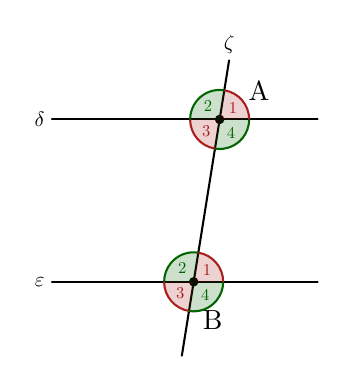
\begin{tikzpicture}[scale=.75]
\tkzSetUpLine[line width=1pt,color=black]
\tkzSetUpPoint[fill=black]

\tkzDefPoints{0/0/A,4.5/0/AA,0/-2.75/B,4.5/-2.75/BB,3/1/C,2.2/-4/CC}

\tkzInterLL(A,AA)(C,CC) \tkzGetPoint{X}
\tkzInterLL(B,BB)(C,CC) \tkzGetPoint{Y}

\tkzDrawSegments[line width=0.75pt](A,AA B,BB C,CC)

\tkzDrawPoints[size=3](X,Y)
\tkzLabelPoint[left,scale=0.75](A){$\rm \delta$}
\tkzLabelPoint[left,scale=0.75](B){$\rm \varepsilon$}
\tkzLabelPoint[above,scale=0.75](C){$\rm \zeta$}

\tkzLabelPoint[xshift=0.5cm,yshift=0.6cm](X){$\rm A$}
\tkzLabelPoint[xshift=0.24cm,yshift=-0.24cm](Y){$\rm B$}

\tkzFillAngles[fill=RedClr,fill opacity=0.2,size=.5](AA,X,C A,X,CC BB,Y,C B,Y,CC)
\tkzMarkAngles[line width=0.75pt,color=RedClr,size=.5](AA,X,C A,X,CC BB,Y,C B,Y,CC)

\tkzFillAngles[fill=AngleClr,fill opacity=0.2,size=.5](C,X,A CC,X,AA C,Y,B CC,Y,BB)
\tkzMarkAngles[line width=0.75pt,color=AngleClr,size=.5](C,X,A CC,X,AA C,Y,B CC,Y,BB)


\tkzLabelAngles[AngleClr,pos=0.5,scale=0.6](C,X,A){$2$}
\tkzLabelAngles[AngleClr,pos=0.5,scale=0.6](CC,X,AA){$4$}
\tkzLabelAngles[AngleClr,pos=0.5,scale=0.6](C,Y,B){$2$}
\tkzLabelAngles[AngleClr,pos=0.5,scale=0.6](CC,Y,BB){$4$}

\tkzLabelAngles[RedClr,pos=0.5,scale=0.6](BB,Y,C){$1$}
\tkzLabelAngles[RedClr,pos=0.5,scale=0.6](B,Y,CC){$3$}
\tkzLabelAngles[RedClr,pos=0.5,scale=0.6](AA,X,C){$1$}
\tkzLabelAngles[RedClr,pos=0.5,scale=0.6](A,X,CC){$3$}



\end{tikzpicture}

\end{document}
